\documentclass[11pt]{article}
\usepackage[margin=0.85in]{geometry}

% Core packages
\usepackage{amsmath,amssymb}
\usepackage{xcolor}
\usepackage{setspace}
\usepackage{enumitem}
\usepackage{float}
\usepackage{placeins}
\usepackage{booktabs}
\usepackage{longtable}
\usepackage{caption}
\usepackage{adjustbox}
\usepackage{array}
\usepackage{multirow}
\usepackage{tabularx}
\usepackage{tikz}
\usepackage[hidelinks]{hyperref}
\captionsetup{hypcap=false}

\usetikzlibrary{arrows.meta, shapes.geometric, positioning, calc, fit, backgrounds}

% Paragraphs
\setlength{\parindent}{1.5em}
\setlength{\parskip}{0.3\baselineskip}
\setstretch{1.12}
\setcounter{tocdepth}{3}
\setcounter{secnumdepth}{3}
\setlist{itemsep=0.15\baselineskip, topsep=0.25\baselineskip, parsep=0pt, partopsep=0pt}
\emergencystretch=3em
\hfuzz=15pt
\hbadness=10000

\makeatletter
\renewcommand\paragraph{\@startsection{paragraph}{4}{\z@}%
  {0.85\baselineskip}%
  {0.25\baselineskip}%
  {\normalfont\normalsize\bfseries}}
\makeatother

\definecolor{ejustblue}{HTML}{1F4E79}
\definecolor{stage}{HTML}{0f4662}
\definecolor{inputcolor}{HTML}{2e7d32}
\definecolor{outputcolor}{HTML}{c62828}
\definecolor{processcolor}{HTML}{1565c0}
\definecolor{softblue}{HTML}{E3F2FD}
\definecolor{softgreen}{HTML}{E8F5E9}
\definecolor{softyellow}{HTML}{FFF8E1}
\definecolor{softorange}{HTML}{FFF3E0}
\definecolor{softpurple}{HTML}{F3E5F5}
\definecolor{softred}{HTML}{FFEBEE}
\definecolor{softgray}{HTML}{F5F5F5}

% Stage heading
\newcommand{\stageheading}[2]{%
  \vspace{0.8\baselineskip}%
  \noindent%
  \begin{tikzpicture}
    \node[fill=stage, text=white, minimum width=\textwidth, minimum height=1cm,
          inner sep=6pt, font=\large\bfseries, rounded corners=3pt] {Stage #1: #2};
  \end{tikzpicture}%
  \par\vspace{0.3\baselineskip}%
}

% Input/Output/Process boxes
\newcommand{\inputbox}[1]{%
  \par\vspace{0.3\baselineskip}%
  \noindent\fcolorbox{inputcolor!60}{softgreen!50}{%
    \parbox{0.95\textwidth}{\textcolor{inputcolor}{\textbf{What goes IN:}} #1}%
  }\par\vspace{0.15\baselineskip}%
}

\newcommand{\processbox}[1]{%
  \par\vspace{0.15\baselineskip}%
  \noindent\fcolorbox{processcolor!60}{softblue!50}{%
    \parbox{0.95\textwidth}{\textcolor{processcolor}{\textbf{What HAPPENS:}} #1}%
  }\par\vspace{0.15\baselineskip}%
}

\newcommand{\outputbox}[1]{%
  \par\vspace{0.15\baselineskip}%
  \noindent\fcolorbox{outputcolor!60}{softred!40}{%
    \parbox{0.95\textwidth}{\textcolor{outputcolor}{\textbf{What comes OUT:}} #1}%
  }\par\vspace{0.3\baselineskip}%
}

\newcommand{\whybox}[1]{%
  \par\vspace{0.15\baselineskip}%
  \noindent\fcolorbox{black!30}{softyellow!60}{%
    \parbox{0.95\textwidth}{\textbf{Why this stage matters:} #1}%
  }\par\vspace{0.3\baselineskip}%
}

\begin{document}
\pagenumbering{gobble}
\hypersetup{pageanchor=false}

% ======================================================
% TITLE PAGE
% ======================================================
\begin{titlepage}
\setlength{\parskip}{0pt}
\thispagestyle{empty}
\centering

\vspace*{1.5cm}

{\color{ejustblue}\rule{0.78\textwidth}{1.6pt}\par}
\vspace{0.5cm}
{\huge\bfseries How the System Works\par}
\vspace{0.3cm}
{\LARGE A Step-by-Step Guide\par}
\vspace{0.15cm}
{\Large\itshape from Raw Data to Final Supplier--Buyer Matches\par}
\vspace{0.5cm}
{\color{ejustblue}\rule{0.78\textwidth}{1.6pt}\par}

\vspace{1.2cm}

{\large This document explains in simple language what each stage of the Integrated Fuzzy Supplier--Buyer Evaluation system does. For every stage, it shows:\par}

\vspace{0.6cm}

\begin{minipage}{0.75\textwidth}
\begin{itemize}[leftmargin=2em, itemsep=0.5em]
  \item[\textcolor{inputcolor}{$\blacktriangleright$}] \textbf{What goes IN} --- the data the stage receives
  \item[\textcolor{processcolor}{$\blacktriangleright$}] \textbf{What HAPPENS} --- the transformation or computation
  \item[\textcolor{outputcolor}{$\blacktriangleright$}] \textbf{What comes OUT} --- the result passed to the next stage
  \item[\textcolor{black}{$\blacktriangleright$}] \textbf{A concrete example} --- with small numbers you can follow by hand
\end{itemize}
\end{minipage}

\vspace{2cm}

{\large\bfseries An Integrated Fuzzy Approach for Supplier--Buyer\\Evaluation, Scoring, and Selection\par}

\vspace{1cm}
{\large September 2026\par}

\end{titlepage}

% ======================================================
% TABLE OF CONTENTS
% ======================================================
\newpage
\pagenumbering{roman}
\hypersetup{pageanchor=true}
\begingroup
\setlength{\parskip}{0pt}
\setstretch{1}
\tableofcontents
\endgroup
\newpage
\pagenumbering{arabic}

% ======================================================
% SECTION 1: THE BIG PICTURE
% ======================================================
\section{The Big Picture}

\subsection{What Problem Are We Solving?}

Imagine a factory (the \textbf{buyer}) that needs to choose which raw material suppliers to work with. At the same time, each \textbf{supplier} also chooses which buyers it wants to prioritize --- because suppliers have limited capacity and prefer buyers who pay on time, order predictably, and are easy to work with.

Most existing systems only look at one side: the buyer picks the best supplier. But that ignores the fact that the supplier might not want to work with that buyer. Our system evaluates \textbf{both sides at the same time} --- the buyer rates the suppliers, the supplier rates the buyers, and then we \textbf{match} them so that both parties are happy.

\subsection{What Does the System Actually Do?}

Think of the system as a pipeline with nine stations. Raw data enters at the beginning, gets cleaned, scored, predicted, matched, and recorded, and at the end you get a report telling you which supplier should work with which buyer.

Here is the flow at the highest level:

\begin{center}
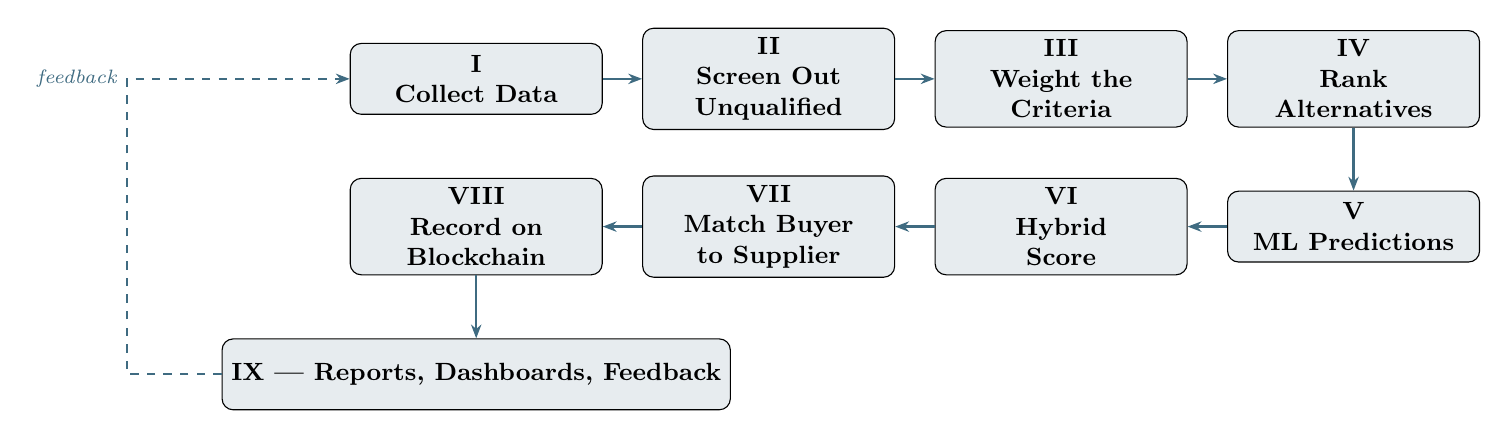
\begin{tikzpicture}[
  node distance=0.5cm,
  stage/.style={draw, rounded corners, fill=stage!10, text=black,
                minimum width=3.2cm, minimum height=0.9cm,
                font=\small\bfseries, align=center},
  arrow/.style={-{Stealth[length=5pt]}, thick, stage!80}
]
  \node[stage] (s1) {I\\Collect Data};
  \node[stage, right=of s1] (s2) {II\\Screen Out\\Unqualified};
  \node[stage, right=of s2] (s3) {III\\Weight the\\Criteria};
  \node[stage, right=of s3] (s4) {IV\\Rank\\Alternatives};

  \node[stage, below=0.8cm of s4] (s5) {V\\ML Predictions};
  \node[stage, left=of s5] (s6) {VI\\Hybrid\\Score};
  \node[stage, left=of s6] (s7) {VII\\Match Buyer\\to Supplier};
  \node[stage, left=of s7] (s8) {VIII\\Record on\\Blockchain};

  \node[stage, below=0.8cm of s8, minimum width=4cm] (s9) {IX --- Reports, Dashboards, Feedback};

  \draw[arrow] (s1) -- (s2);
  \draw[arrow] (s2) -- (s3);
  \draw[arrow] (s3) -- (s4);
  \draw[arrow] (s4) -- (s5);
  \draw[arrow] (s5) -- (s6);
  \draw[arrow] (s6) -- (s7);
  \draw[arrow] (s7) -- (s8);
  \draw[arrow] (s8) -- (s9);
  \draw[arrow, dashed] (s9.west) -- ++(-1.2,0) |- (s1.west) node[midway, left, font=\scriptsize\itshape] {feedback};
\end{tikzpicture}
\end{center}

The dashed arrow at the bottom shows that the system \textbf{learns}: after each cycle of matching, real-world outcomes are fed back to improve the next evaluation round.

\subsection{Why Both Sides? --- A Simple Analogy}

Think of a dating app. If only one person swipes right, there is no match. Both people have to like each other for the match to work. Our system is the same idea applied to business:

\begin{center}
\begin{tabular}{ccc}
\textbf{Buyer evaluates Suppliers} & $\longleftrightarrow$ & \textbf{Supplier evaluates Buyers} \\
``Which supplier is best for me?'' & & ``Which buyer is best for me?'' \\
\end{tabular}
\end{center}

Only when \textbf{both} sides rank each other highly does the system propose a match.

% ======================================================
% SECTION 2: THE CRITERIA
% ======================================================
\section{The Evaluation Criteria --- What We Measure}

Before anything is calculated, we need to know what \textit{matters}. The system uses two separate lists of criteria: one for evaluating suppliers and one for evaluating buyers.

\subsection{How a Buyer Evaluates Suppliers (8 Criteria)}

When a buyer looks at a potential supplier, they care about:

\begin{center}
\small
\begin{tabular}{clp{8cm}}
\toprule
\textbf{\#} & \textbf{Criterion} & \textbf{What It Means (in plain words)} \\
\midrule
1 & Quality Performance & Does the supplier make good products with few defects? \\
2 & Delivery Performance & Does the supplier deliver on time and in full? \\
3 & Cost Competitiveness & Are the prices fair? (Lower is better --- this is the only ``cost'' criterion.) \\
4 & Financial Stability & Is the supplier financially healthy and not at risk of going bankrupt? \\
5 & Technical Capability & Can the supplier solve technical problems and innovate? \\
6 & Compliance \& Sustainability & Does the supplier follow environmental and safety laws? \\
7 & Systems Integration & Can the supplier's IT systems talk to the buyer's systems? \\
8 & Experience \& Track Record & Has the supplier done this kind of work before, successfully? \\
\bottomrule
\end{tabular}
\end{center}

Notice that 7 out of 8 criteria are ``benefit'' criteria (higher is better), and only \textbf{Cost Competitiveness} is a ``cost'' criterion (lower is better). This distinction matters later when we normalize and rank.

\subsection{How a Supplier Evaluates Buyers (9 Criteria)}

When a supplier looks at a potential buyer, they care about:

\begin{center}
\small
\begin{tabular}{clp{8cm}}
\toprule
\textbf{\#} & \textbf{Criterion} & \textbf{What It Means (in plain words)} \\
\midrule
1 & Financial Stability \& Creditworthiness & Can the buyer actually pay? Are they financially safe? \\
2 & Payment Performance & Does the buyer pay invoices on time, without disputes? \\
3 & Order Volume \& Growth Potential & Does the buyer order a lot, and is their business growing? \\
4 & Demand Stability \& Predictability & Are the buyer's orders steady and predictable, or chaotic? \\
5 & Responsiveness \& Collaboration & Is the buyer easy to communicate with? Do they solve problems together? \\
6 & Compliance \& Regulatory Standards & Does the buyer follow data privacy and ethical business rules? \\
7 & Tech.\ Sophistication \& Sys.\ Integ. & Can the buyer send orders electronically and share data digitally? \\
8 & Market Reputation \& Brand Impact & Will working with this buyer make the supplier look good? \\
9 & Long-Term Strategic Value & Is this buyer worth keeping for years, with growth and innovation potential? \\
\bottomrule
\end{tabular}
\end{center}

All 9 buyer criteria are ``benefit'' criteria: higher is always better.

% ======================================================
% SECTION 3: THE NINE STAGES IN DETAIL
% ======================================================
\section{The Nine Stages --- Step by Step}

Now let us walk through every stage. We will follow a small running example with \textbf{3 suppliers} being evaluated by a buyer using \textbf{4 criteria} (a simplified version to keep the numbers readable).

% --------------------------------------------------
% STAGE I
% --------------------------------------------------
\stageheading{I}{Data Acquisition and Preprocessing}

\whybox{You cannot evaluate anyone without data. This stage collects scores for every supplier and every buyer on every criterion, and then makes the numbers comparable.}

\inputbox{Raw performance scores for each entity on each criterion. Scores are entered on a 1--10 scale, where 1 is terrible and 10 is excellent. They can come from manual entry, historical procurement records, or synthetic (test) data.}

\textbf{Example.} A buyer scores three suppliers on four criteria:

\begin{center}
\begin{tabular}{lcccc}
\toprule
 & Quality & Delivery & Cost & Tech.\ Capability \\
\midrule
Supplier A & 9 & 7 & 3 & 8 \\
Supplier B & 6 & 9 & 7 & 5 \\
Supplier C & 8 & 6 & 5 & 9 \\
\bottomrule
\end{tabular}
\captionof{table}{Raw decision matrix --- the starting point of everything.}
\end{center}

\processbox{The raw scores are on the same 1--10 scale, but they are not comparable yet because ``Cost'' works in reverse (lower is better). Normalization fixes this. Two normalization methods are used:\smallskip

\textbf{Min-max normalization} (used by AHP, Fuzzy AHP, and VIKOR): rescales each column so that the best value becomes 1 and the worst becomes 0.
\begin{itemize}
  \item For benefit criteria: $\displaystyle r_{ij} = \frac{x_{ij} - \min(x_j)}{\max(x_j) - \min(x_j)}$
  \item For cost criteria: $\displaystyle r_{ij} = \frac{\max(x_j) - x_{ij}}{\max(x_j) - \min(x_j)}$
\end{itemize}

\textbf{Vector normalization} (used by TOPSIS): divides each value by the length of its column vector: $\displaystyle r_{ij} = \frac{x_{ij}}{\sqrt{\sum_{k} x_{kj}^2}}$
}

\textbf{Example (min-max).} For the Quality column: $\min=6$, $\max=9$, range$=3$.
\begin{itemize}
  \item Supplier A: $(9-6)/3 = 1.00$
  \item Supplier B: $(6-6)/3 = 0.00$
  \item Supplier C: $(8-6)/3 = 0.67$
\end{itemize}
For the Cost column (reversed because lower cost is better): $\min=3$, $\max=7$, range$=4$.
\begin{itemize}
  \item Supplier A: $(7-3)/4 = 1.00$ \quad (cost 3 is the best, so it gets 1.00)
  \item Supplier B: $(7-7)/4 = 0.00$ \quad (cost 7 is the worst, so it gets 0.00)
  \item Supplier C: $(7-5)/4 = 0.50$
\end{itemize}

\begin{center}
\begin{tabular}{lcccc}
\toprule
 & Quality & Delivery & Cost & Tech.\ Capability \\
\midrule
Supplier A & 1.00 & 0.33 & 1.00 & 0.75 \\
Supplier B & 0.00 & 1.00 & 0.00 & 0.00 \\
Supplier C & 0.67 & 0.00 & 0.50 & 1.00 \\
\bottomrule
\end{tabular}
\captionof{table}{Normalized decision matrix --- all values are now between 0 and 1, and higher is always better.}
\end{center}

\outputbox{A normalized decision matrix where every value is between 0 and 1, all criteria point the same direction (higher = better), and different measurement units are eliminated.}

% --------------------------------------------------
% STAGE II
% --------------------------------------------------
\stageheading{II}{Screening via Binary Qualification Gates}

\whybox{Some suppliers or buyers should not even be considered. If a supplier does not have a required safety certification, it does not matter how good their price is --- they are disqualified. This stage removes unqualified entities \textit{before} the expensive scoring begins, saving time and ensuring legal compliance.}

\inputbox{The full list of entities (suppliers or buyers) plus a set of \textbf{pass/fail requirements}. These are yes-or-no questions, not scored criteria. Examples: ``Has ISO 9001 certification?'', ``Meets minimum order capacity of 500 units?'', ``Passed environmental audit?''}

\textbf{Example.} Three gate criteria applied to our suppliers:

\begin{center}
\begin{tabular}{lccc}
\toprule
 & ISO 9001? & Capacity $\geq$ 500? & Env.\ Audit Passed? \\
\midrule
Supplier A & \textcolor{inputcolor}{\checkmark} Yes & \textcolor{inputcolor}{\checkmark} Yes & \textcolor{inputcolor}{\checkmark} Yes \\
Supplier B & \textcolor{inputcolor}{\checkmark} Yes & \textcolor{outputcolor}{$\times$} No (350 only) & \textcolor{inputcolor}{\checkmark} Yes \\
Supplier C & \textcolor{inputcolor}{\checkmark} Yes & \textcolor{inputcolor}{\checkmark} Yes & \textcolor{inputcolor}{\checkmark} Yes \\
\bottomrule
\end{tabular}
\captionof{table}{Binary gate screening results.}
\end{center}

\processbox{Every entity is checked against every gate. If it fails \textbf{any single gate}, it is removed from the pool entirely. There is no partial credit --- it is strictly pass or fail.}

\outputbox{A reduced list containing only the qualified entities. In the example, Supplier B is eliminated because its capacity is below the minimum. Only Suppliers A and C continue to Stage III.}

% --------------------------------------------------
% STAGE III
% --------------------------------------------------
\stageheading{III}{Criteria Weighting --- How Important Is Each Criterion?}

\whybox{Not all criteria are equally important. A hospital buying surgical equipment cares far more about Quality than about Cost. A discount retailer might care more about Cost. This stage determines the \textbf{importance weight} of each criterion, so the ranking reflects the decision-maker's priorities.}

\inputbox{An expert's judgment about the relative importance of each criterion. This judgment can be expressed in three ways (the user chooses which one to use).}

The system supports three weighting methods:

\subsubsection{Method 1: Direct Weighting}

The simplest approach. The expert directly assigns a number to each criterion:

\begin{center}
\begin{tabular}{lccc}
\toprule
Criterion & Raw Weight & $\div$ Sum & Normalized Weight \\
\midrule
Quality & 10 & $10/25$ & 0.40 \\
Delivery & 7 & $7/25$ & 0.28 \\
Cost & 5 & $5/25$ & 0.20 \\
Tech.\ Capability & 3 & $3/25$ & 0.12 \\
\midrule
\textbf{Sum} & \textbf{25} & & \textbf{1.00} \\
\bottomrule
\end{tabular}
\captionof{table}{Direct weighting: raw numbers are normalized to sum to 1.}
\end{center}

The weights always sum to 1. This tells us: Quality counts for 40\% of the final score, Delivery for 28\%, and so on.

\subsubsection{Method 2: AHP --- Pairwise Comparison}

Instead of assigning direct numbers, the expert compares criteria \textit{two at a time}: ``How much more important is Quality than Delivery?'' The answer uses a 1--9 scale:

\begin{center}
\small
\begin{tabular}{cl}
\toprule
\textbf{Value} & \textbf{Meaning} \\
\midrule
1 & Equally important \\
3 & Moderately more important \\
5 & Strongly more important \\
7 & Very strongly more important \\
9 & Extremely more important \\
\bottomrule
\end{tabular}
\end{center}

\textbf{Example.} An expert fills in the upper triangle of a comparison matrix:

\begin{center}
\begin{tabular}{lcccc}
\toprule
 & Quality & Delivery & Cost & Tech \\
\midrule
Quality & 1 & 3 & 5 & 7 \\
Delivery & 1/3 & 1 & 3 & 5 \\
Cost & 1/5 & 1/3 & 1 & 3 \\
Tech & 1/7 & 1/5 & 1/3 & 1 \\
\bottomrule
\end{tabular}
\captionof{table}{AHP pairwise comparison matrix. Note: the lower triangle is just the reciprocal of the upper triangle (e.g., if Quality vs Delivery = 3, then Delivery vs Quality = 1/3).}
\end{center}

\processbox{
\begin{enumerate}[leftmargin=2em]
  \item \textbf{Normalize each column} by dividing every cell by the column sum.
  \item \textbf{Average each row} to get the weight for that criterion.
  \item \textbf{Consistency check}: calculate the Consistency Ratio ($CR$). If $CR > 0.10$, the expert's judgments are contradictory and must be revised. For example, saying ``Quality $\gg$ Cost'' and ``Cost $\gg$ Quality'' at the same time would fail this check.
\end{enumerate}
}

\outputbox{A weight vector like $[0.56,\ 0.26,\ 0.12,\ 0.06]$ plus a Consistency Ratio confirming the judgments are logical.}

\subsubsection{Method 3: Fuzzy AHP --- Handling Uncertainty}

In real life, an expert might not be sure whether Quality is ``3 times'' or ``4 times'' more important than Delivery. Fuzzy AHP handles this uncertainty by replacing each crisp number with a \textbf{triangle of three numbers} $(l, m, u)$ representing the \textit{minimum}, \textit{most likely}, and \textit{maximum} possible value:

\begin{center}
\small
\begin{tabular}{lc}
\toprule
\textbf{Linguistic Term} & \textbf{Fuzzy Number $(l, m, u)$} \\
\midrule
Equally important & (1, 1, 1) \\
Weakly more important & (1, 2, 3) \\
Moderately more important & (2, 3, 4) \\
Strongly more important & (3, 4, 5) \\
Very strongly more important & (4, 5, 6) \\
Extremely more important & (5, 6, 7) \\
\bottomrule
\end{tabular}
\captionof{table}{Fuzzy linguistic scale. Instead of saying ``3'', the expert says ``moderately more important'' which translates to the range (2, 3, 4).}
\end{center}

\processbox{
\begin{enumerate}[leftmargin=2em]
  \item Build a fuzzy pairwise comparison matrix using triangular fuzzy numbers.
  \item Compute \textbf{fuzzy geometric means} for each row (Buckley's method).
  \item \textbf{Defuzzify}: convert each fuzzy weight back to a single crisp number by averaging its three components: $w = (l + m + u) / 3$.
  \item Normalize so the weights sum to 1.
\end{enumerate}
}

\outputbox{A weight vector similar to AHP's, but derived from uncertain linguistic judgments rather than precise numbers. Typical output: $[0.52,\ 0.28,\ 0.13,\ 0.07]$.}

% --------------------------------------------------
% STAGE IV
% --------------------------------------------------
\stageheading{IV}{Alternative Ranking --- Scoring Each Supplier/Buyer}

\whybox{Now that we know the weights (from Stage III) and the normalized scores (from Stage I), we can compute a single overall score for each entity and rank them from best to worst. The system runs \textbf{multiple ranking methods} on the same data and compares results to ensure the ranking is robust --- if different methods agree, we have high confidence in the result.}

\inputbox{The normalized decision matrix from Stage I + the criteria weights from Stage III.}

The system uses three ranking methods in parallel:

\subsubsection{Method A: AHP-Based Weighted Sum (Simple)}

This is the most intuitive method. Multiply each normalized score by its weight and add them up:

\[
\text{Score}_i = \sum_{j=1}^{n} w_j \times r_{ij}
\]

\textbf{Example.} Using weights $[0.40, 0.28, 0.20, 0.12]$ and the normalized matrix:

\begin{center}
\begin{tabular}{lccccc}
\toprule
 & Quality & Delivery & Cost & Tech & \textbf{Score} \\
 & ($\times 0.40$) & ($\times 0.28$) & ($\times 0.20$) & ($\times 0.12$) & \\
\midrule
Supplier A & $1.00 \times 0.40$ & $0.33 \times 0.28$ & $1.00 \times 0.20$ & $0.75 \times 0.12$ & \textbf{0.783} \\
Supplier C & $0.67 \times 0.40$ & $0.00 \times 0.28$ & $0.50 \times 0.20$ & $1.00 \times 0.12$ & \textbf{0.488} \\
\bottomrule
\end{tabular}
\captionof{table}{AHP weighted sum scoring. Supplier A scores higher.}
\end{center}

\subsubsection{Method B: TOPSIS --- Distance to the Ideal Solution}

TOPSIS asks: ``How close is each supplier to the \textit{perfect} supplier, and how far is it from the \textit{worst possible} supplier?''

\processbox{
\begin{enumerate}[leftmargin=2em]
  \item \textbf{Build the weighted normalized matrix}: $v_{ij} = w_j \times r_{ij}$
  \item \textbf{Find the Positive Ideal Solution (PIS)}: the best value in each column.
  \item \textbf{Find the Negative Ideal Solution (NIS)}: the worst value in each column.
  \item \textbf{Measure the Euclidean distance} from each supplier to PIS ($D^+$) and NIS ($D^-$).
  \item \textbf{Compute the closeness coefficient}: $CC_i = D_i^- / (D_i^+ + D_i^-)$. A value close to 1 means the supplier is near-perfect; close to 0 means near-worst.
\end{enumerate}
}

\textbf{Intuition.} Think of it geometrically: every supplier is a point in multi-dimensional space. PIS is the ``dream supplier'' point. NIS is the ``nightmare supplier'' point. TOPSIS picks the supplier closest to the dream and farthest from the nightmare.

\subsubsection{Method C: VIKOR --- Compromise Ranking}

VIKOR is different from TOPSIS. Instead of measuring geometric distance, it asks two questions:

\begin{enumerate}
  \item \textbf{Group utility ($S$)}: How good is the supplier \textit{overall across all criteria}? (Sum of all gaps from the ideal.)
  \item \textbf{Individual regret ($R$)}: What is the supplier's \textit{worst single weakness}? (The largest gap on any one criterion.)
\end{enumerate}

These two measures are combined into a compromise index $Q$:

\[
Q_i = v \times \frac{S_i - S^*}{S^- - S^*} + (1-v) \times \frac{R_i - R^*}{R^- - R^*}
\]

The parameter $v$ (set to 0.5 by default) controls the balance:
\begin{itemize}
  \item $v = 1.0$: Purely utility-focused --- pick the supplier that is best on average, even if it has one weak area.
  \item $v = 0.0$: Purely regret-averse --- pick the supplier with no severe weaknesses, even if its average is lower.
  \item $v = 0.5$: A balanced compromise between the two.
\end{itemize}

VIKOR also checks two \textbf{compromise conditions} to verify that the top-ranked supplier is truly the best, not just marginally ahead. If the conditions are not met, VIKOR reports a \textit{set} of compromise solutions rather than a single winner.

\outputbox{For \textbf{each} ranking method, a ranked list of all qualified entities with their scores. The system also flags VIKOR compromise solutions. Since both buyer and supplier evaluations are performed, there are \textbf{two parallel sets of rankings} --- one from the buyer's side and one from the supplier's side.}

\begin{center}
\begin{tabular}{clc|clc}
\toprule
\multicolumn{3}{c|}{\textbf{Buyer's Ranking of Suppliers}} & \multicolumn{3}{c}{\textbf{Supplier's Ranking of Buyers}} \\
Rank & Supplier & Score & Rank & Buyer & Score \\
\midrule
1 & Supplier A & 0.783 & 1 & Buyer X & 0.812 \\
2 & Supplier C & 0.488 & 2 & Buyer Y & 0.654 \\
  &            &       & 3 & Buyer Z & 0.523 \\
\bottomrule
\end{tabular}
\captionof{table}{Two parallel ranking lists --- this is what makes the system \textit{bi-directional}.}
\end{center}

% --------------------------------------------------
% STAGE V
% --------------------------------------------------
\stageheading{V}{Machine Learning --- Predicting Future Performance}

\whybox{MCDM scores reflect how a supplier performs \textit{today}. But what about tomorrow? A supplier with great scores now might be declining. A supplier with mediocre scores might be rapidly improving. Machine Learning uses \textbf{historical patterns} to predict future performance, adding a forward-looking dimension that static scoring cannot provide.}

\inputbox{Historical performance data: multiple evaluation periods for each entity. For example, Supplier A's quality scores over the last 8 quarters: $[7, 7, 8, 8, 8, 9, 9, 9]$ --- showing an upward trend.}

\processbox{
\begin{enumerate}[leftmargin=2em]
  \item \textbf{Split the data} into training (past data) and testing (recent data) sets.
  \item \textbf{Train predictive models} (Random Forest, Gradient Boosting, etc.) to learn the relationship between historical performance features and future outcomes.
  \item \textbf{Generate predictions}: for each entity, predict what their performance scores will look like in the next period.
  \item \textbf{Validate}: compare predictions to actual outcomes on the test set to measure accuracy.
\end{enumerate}
}

\textbf{Example.} The ML model might predict:

\begin{center}
\begin{tabular}{lcccc}
\toprule
 & Quality & Delivery & Cost & Tech \\
 & (predicted) & (predicted) & (predicted) & (predicted) \\
\midrule
Supplier A & 9.2 & 7.5 & 3.1 & 8.3 \\
Supplier C & 7.5 & 6.8 & 5.2 & 9.5 \\
\bottomrule
\end{tabular}
\captionof{table}{ML-predicted performance scores for the next evaluation period.}
\end{center}

\outputbox{Predicted future performance scores for each entity, plus model accuracy metrics (how reliable these predictions are).}

% --------------------------------------------------
% STAGE VI
% --------------------------------------------------
\stageheading{VI}{Hybrid Scoring --- Combining Expert Judgment with ML Predictions}

\whybox{Expert judgment (from FAHP) captures domain knowledge. ML predictions capture data patterns. Neither alone is perfect. Combining them gives a more balanced and accurate final score.}

\inputbox{Two sets of scores for each entity: (1) MCDM scores from Stage IV based on expert-weighted criteria, and (2) ML-predicted scores from Stage V.}

\processbox{The two scores are blended using a tunable parameter $\alpha$:

\[
\text{Score}_{\text{hybrid}} = \alpha \times \text{Score}_{\text{MCDM}} + (1 - \alpha) \times \text{Score}_{\text{ML}}
\]

If $\alpha = 0.7$, the expert judgment counts for 70\% and the ML prediction counts for 30\%. The user can adjust $\alpha$ depending on how much they trust the ML predictions.
}

\textbf{Example} ($\alpha = 0.7$):

\begin{center}
\begin{tabular}{lcccc}
\toprule
 & MCDM Score & ML Score & Hybrid Score & Rank \\
\midrule
Supplier A & 0.783 & 0.810 & $0.7 \times 0.783 + 0.3 \times 0.810 = \mathbf{0.791}$ & 1 \\
Supplier C & 0.488 & 0.620 & $0.7 \times 0.488 + 0.3 \times 0.620 = \mathbf{0.528}$ & 2 \\
\bottomrule
\end{tabular}
\captionof{table}{Hybrid scoring blends MCDM and ML into one final score.}
\end{center}

\outputbox{A single hybrid score for each entity that captures both expert knowledge and data-driven prediction.}

% --------------------------------------------------
% STAGE VII
% --------------------------------------------------
\stageheading{VII}{Matching --- Pairing Buyers with Suppliers}

\whybox{Having ranked both sides independently is not enough. We need to actually \textit{pair} each buyer with a supplier such that \textbf{both parties are reasonably satisfied}. This is the core novelty of the project --- it treats procurement as a two-sided matching problem, like the Nobel Prize-winning Gale-Shapley algorithm used in medical residency matching.}

\inputbox{Two ranked preference lists: each buyer's ranking of suppliers (from Stage IV/VI) and each supplier's ranking of buyers (from Stage IV/VI).}

\textbf{Example.} Suppose we have 2 buyers and 3 suppliers:

\begin{center}
\begin{tabular}{ll}
\toprule
\textbf{Buyer preferences} & \textbf{Supplier preferences} \\
\midrule
Buyer X: $A \succ C \succ B$ & Supplier A: $Y \succ X$ \\
Buyer Y: $A \succ B \succ C$ & Supplier B: $X \succ Y$ \\
                              & Supplier C: $X \succ Y$ \\
\bottomrule
\end{tabular}
\captionof{table}{Preference lists. $A \succ C$ means ``prefers A over C''.}
\end{center}

\processbox{
\begin{enumerate}[leftmargin=2em]
  \item \textbf{Initial matching} using the Gale-Shapley Deferred Acceptance Algorithm:
  \begin{itemize}
    \item Round 1: Both buyers propose to Supplier A (their first choice).
    \item Supplier A prefers Buyer Y, so Buyer Y gets tentatively matched with A, and Buyer X is rejected.
    \item Round 2: Buyer X proposes to Supplier C (their next choice). Supplier C accepts.
    \item Result: Buyer X $\leftrightarrow$ Supplier C, Buyer Y $\leftrightarrow$ Supplier A.
  \end{itemize}
  \item \textbf{Stability check}: Is there any buyer--supplier pair who would both prefer to be matched with each other over their current partners? If not, the matching is \textit{stable} --- no one has an incentive to break their assignment.
  \item \textbf{RL optimization}: A Reinforcement Learning agent explores alternative matchings over time, learning from actual relationship outcomes (did the pairing work well?) to propose even better matches in future cycles.
\end{enumerate}
}

\outputbox{A set of stable buyer--supplier pairings where no pair has a mutual incentive to switch.}

\begin{center}
\begin{tabular}{cc}
\toprule
\textbf{Buyer} & \textbf{Matched Supplier} \\
\midrule
Buyer X & Supplier C \\
Buyer Y & Supplier A \\
\bottomrule
\end{tabular}
\captionof{table}{Final stable matching output.}
\end{center}

% --------------------------------------------------
% STAGE VIII
% --------------------------------------------------
\stageheading{VIII}{Blockchain --- Tamper-Proof Records}

\whybox{In business procurement, disputes happen. A supplier might claim ``my quality score was 9, not 7.'' A buyer might deny receiving a delivery. Blockchain provides an \textbf{immutable ledger} --- once data is recorded, it cannot be secretly changed by anyone. This creates trust between parties who may not fully trust each other.}

\inputbox{All evaluation data from previous stages: raw scores, normalized scores, criteria weights, MCDM rankings, ML predictions, hybrid scores, and matching results.}

\processbox{
\begin{enumerate}[leftmargin=2em]
  \item \textbf{Hash and record} each evaluation event on a blockchain ledger (e.g., Hyperledger Fabric). This creates a permanent, timestamped, cryptographically signed record.
  \item \textbf{Smart contracts} automatically enforce rules: for example, a contract might require that a supplier's quality score must be verified by an independent auditor before it is recorded.
  \item \textbf{Access control} ensures that only authorized participants can view or submit data, while auditors and regulators can verify records without modifying them.
\end{enumerate}
}

Think of it as a notarized document that everyone can verify but nobody can forge.

\outputbox{An auditable, tamper-proof record of every evaluation decision. Any participant can verify: ``At time $T$, using weights $W$, with scores $X$, the system computed ranking $R$ and matching $M$.'' No one can alter this after the fact.}

% --------------------------------------------------
% STAGE IX
% --------------------------------------------------
\stageheading{IX}{Output, Monitoring, and Feedback}

\whybox{The system does not stop after one matching cycle. In real procurement, relationships evolve. A supplier that was great last year might be declining. The feedback loop captures real-world outcomes and uses them to improve the next evaluation cycle --- making the system smarter over time.}

\inputbox{Analysis results from all previous stages, plus real-world outcome data from the period since the last evaluation (actual delivery performance, payment behavior, quality incidents, etc.).}

\processbox{
\begin{enumerate}[leftmargin=2em]
  \item \textbf{Generate reports}: Excel workbooks with ranked lists, executive summaries of top entities, and bar charts/scatter plots visualizing the results.
  \item \textbf{Display dashboards}: Interactive views showing scores, rankings, and how they change over time.
  \item \textbf{Feedback loop}: Compare predictions from Stage V with actual outcomes. Retrain the ML models with the new data. Update the RL agent's matching strategy based on whether the pairings worked well. Optionally adjust criteria weights if some criteria turn out to be more predictive of success than others.
\end{enumerate}
}

\outputbox{
\begin{itemize}
  \item Styled Excel report with one sheet per method--scheme combination
  \item Top-10 bar charts per method
  \item Cross-scheme scatter comparison plots
  \item Performance trend dashboards
  \item Updated ML models and RL policies ready for the next cycle
\end{itemize}
}

\textbf{The cycle repeats.} The dashed arrow in the pipeline diagram goes from Stage IX back to Stage I, forming a continuous improvement loop.

% ======================================================
% SECTION 4: PUTTING IT ALL TOGETHER
% ======================================================
\section{Putting It All Together --- End-to-End Example}

Let us trace a complete cycle with a concrete scenario.

\begin{center}
\small
\begin{tabularx}{\textwidth}{c >{\raggedright\arraybackslash}p{2.8cm} >{\raggedright\arraybackslash}X}
\toprule
\textbf{Stage} & \textbf{What happens} & \textbf{Concrete output} \\
\midrule
I & Buyer scores 50 suppliers on 8 criteria (1--10). Suppliers score 10 buyers on 9 criteria. & Two raw decision matrices: $50 \times 8$ and $10 \times 9$. \\
\addlinespace
II & 7 suppliers fail ISO certification gate, 2 fail capacity gate. & 41 qualified suppliers remain. All 10 buyers pass. \\
\addlinespace
III & Procurement manager fills AHP pairwise matrix. $CR = 0.04$ (consistent). & Weight vector: Quality 28\%, Delivery 22\%, Cost 18\%, $\ldots$ \\
\addlinespace
IV & AHP, TOPSIS, and VIKOR run on both sides. & 41 suppliers ranked (buyer side). 10 buyers ranked (supplier side). VIKOR identifies 2 compromise suppliers. \\
\addlinespace
V & Random Forest trained on 3 years of historical data. & Predicted scores for next quarter. Model accuracy: 87\%. \\
\addlinespace
VI & Hybrid blend at $\alpha = 0.7$. & Adjusted scores for all 41 suppliers and 10 buyers. \\
\addlinespace
VII & Gale-Shapley matches buyers to suppliers. RL agent fine-tunes. & 10 stable buyer--supplier pairs. \\
\addlinespace
VIII & All evaluation data recorded on Hyperledger Fabric. & 10 blockchain transactions, each containing evaluation hash. \\
\addlinespace
IX & Excel report generated. Dashboard updated. ML retrained with new data from this quarter. & 15-sheet workbook, 8 charts, updated ML model, RL policy. \\
\bottomrule
\end{tabularx}
\captionof{table}{Complete end-to-end trace of the nine-stage pipeline.}
\end{center}

% ======================================================
% SECTION 5: KEY DIFFERENCES FROM TRADITIONAL APPROACHES
% ======================================================
\section{What Makes This System Different}

\begin{center}
\begin{tabularx}{\textwidth}{>{\raggedright\arraybackslash}p{3.5cm} >{\raggedright\arraybackslash}X >{\raggedright\arraybackslash}X}
\toprule
\textbf{Feature} & \textbf{Traditional Systems} & \textbf{Our System} \\
\midrule
Evaluation direction & Buyer evaluates suppliers only (one-way). & Both sides evaluate each other (two-way). \\
\addlinespace
Scoring method & One MCDM method at a time. & Three methods (AHP, TOPSIS, VIKOR) run in parallel for cross-validation. \\
\addlinespace
Uncertainty handling & Uses crisp numbers only. & Fuzzy AHP captures ``I am not exactly sure'' judgments. \\
\addlinespace
Forward-looking & Scores reflect today's performance only. & ML predicts tomorrow's performance. \\
\addlinespace
Matching & No matching --- just a ranked list. & Gale-Shapley stable matching pairs buyers with suppliers. \\
\addlinespace
Learning & Static --- same model every time. & RL agent learns and improves over time. \\
\addlinespace
Trust & Data stored in local files or databases (editable). & Blockchain provides tamper-proof records. \\
\bottomrule
\end{tabularx}
\captionof{table}{Comparison of traditional supplier selection systems vs.\ the proposed framework.}
\end{center}

% ======================================================
% CLOSING
% ======================================================
\vspace{1cm}
\begin{center}
\rule{0.6\textwidth}{0.4pt}
\par\vspace{0.3cm}
{\itshape End of Guide}
\end{center}

\end{document}
